\begin{frame}[fragile]{Visualização do construtor da árvore de segmentos}

    \begin{figure}
        \centering

        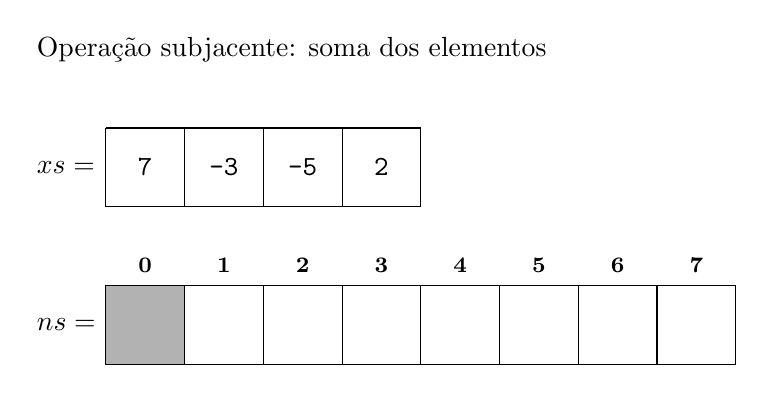
\begin{tikzpicture}
            \node[anchor=west] at (0, 5) { Operação subjacente: soma dos elementos };
            \node[anchor=west] at (0, 3.5) { $xs =$ };
            \node[anchor=west] at (0, 1.5) { $ns =$ };

            \draw[fill=gray!60] (1, 1) rectangle (2, 2);
            \draw (1, 3) grid (5, 4);
            \draw (1, 1) grid (9, 2);

            \node at (1.5, 2.25) { \footnotesize $\mathtt{\mathbf{0}}$ };
            \node at (2.5, 2.25) { \footnotesize $\mathtt{\mathbf{1}}$ };
            \node at (3.5, 2.25) { \footnotesize $\mathtt{\mathbf{2}}$ };
            \node at (4.5, 2.25) { \footnotesize $\mathtt{\mathbf{3}}$ };
            \node at (5.5, 2.25) { \footnotesize $\mathtt{\mathbf{4}}$ };
            \node at (6.5, 2.25) { \footnotesize $\mathtt{\mathbf{5}}$ };
            \node at (7.5, 2.25) { \footnotesize $\mathtt{\mathbf{6}}$ };
            \node at (8.5, 2.25) { \footnotesize $\mathtt{\mathbf{7}}$ };

            \node at (1.5, 3.5) { \tt 7 };
            \node at (2.5, 3.5) { \tt -3 };
            \node at (3.5, 3.5) { \tt -5 };
            \node at (4.5, 3.5) { \tt 2 };
        \end{tikzpicture}
    \end{figure}

\end{frame}

\begin{frame}[fragile]{Visualização do construtor da árvore de segmentos}

    \begin{figure}
        \centering

        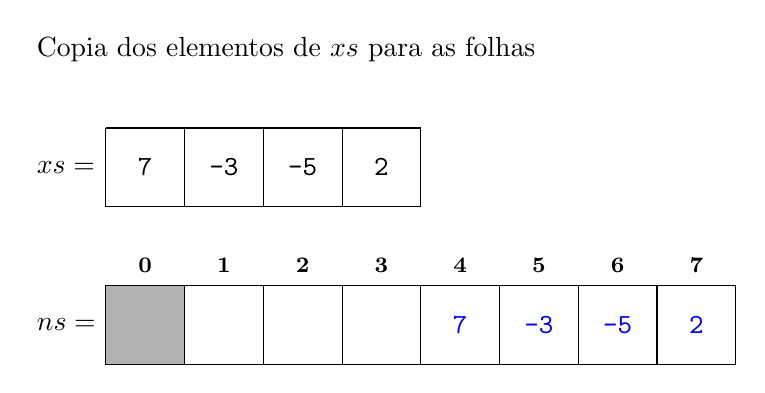
\begin{tikzpicture}
            \node[anchor=west] at (0, 5) { Copia dos elementos de $xs$ para as folhas };
            \node[anchor=west] at (0, 3.5) { $xs =$ };
            \node[anchor=west] at (0, 1.5) { $ns =$ };

            \draw[fill=gray!60] (1, 1) rectangle (2, 2);
            \draw (1, 3) grid (5, 4);
            \draw (1, 1) grid (9, 2);

            \node at (1.5, 2.25) { \footnotesize $\mathtt{\mathbf{0}}$ };
            \node at (2.5, 2.25) { \footnotesize $\mathtt{\mathbf{1}}$ };
            \node at (3.5, 2.25) { \footnotesize $\mathtt{\mathbf{2}}$ };
            \node at (4.5, 2.25) { \footnotesize $\mathtt{\mathbf{3}}$ };
            \node at (5.5, 2.25) { \footnotesize $\mathtt{\mathbf{4}}$ };
            \node at (6.5, 2.25) { \footnotesize $\mathtt{\mathbf{5}}$ };
            \node at (7.5, 2.25) { \footnotesize $\mathtt{\mathbf{6}}$ };
            \node at (8.5, 2.25) { \footnotesize $\mathtt{\mathbf{7}}$ };

            \node at (1.5, 3.5) { \tt 7 };
            \node at (2.5, 3.5) { \tt -3 };
            \node at (3.5, 3.5) { \tt -5 };
            \node at (4.5, 3.5) { \tt 2 };

            \node at (5.5, 1.5) { \tt \textcolor{blue}{7} };
            \node at (6.5, 1.5) { \tt \textcolor{blue}{-3} };
            \node at (7.5, 1.5) { \tt \textcolor{blue}{-5} };
            \node at (8.5, 1.5) { \tt \textcolor{blue}{2} };
        \end{tikzpicture}
    \end{figure}

\end{frame}

\begin{frame}[fragile]{Visualização do construtor da árvore de segmentos}

    \begin{figure}
        \centering

        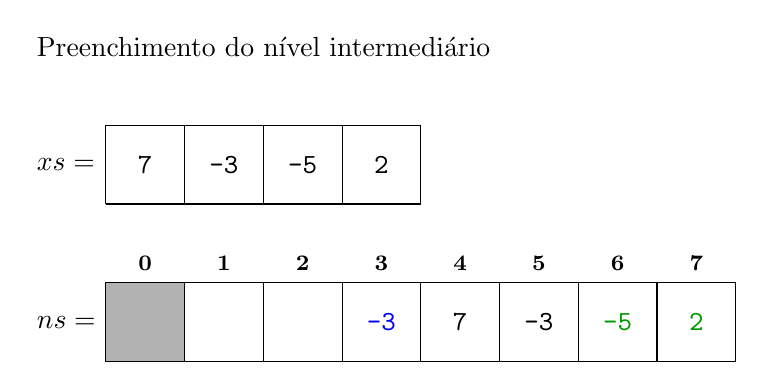
\begin{tikzpicture}
            \node[anchor=west] at (0, 5) { Preenchimento do nível intermediário };
            \node[anchor=west] at (0, 3.5) { $xs =$ };
            \node[anchor=west] at (0, 1.5) { $ns =$ };

            \draw[fill=gray!60] (1, 1) rectangle (2, 2);
            \draw (1, 3) grid (5, 4);
            \draw (1, 1) grid (9, 2);

            \node at (1.5, 2.25) { \footnotesize $\mathtt{\mathbf{0}}$ };
            \node at (2.5, 2.25) { \footnotesize $\mathtt{\mathbf{1}}$ };
            \node at (3.5, 2.25) { \footnotesize $\mathtt{\mathbf{2}}$ };
            \node at (4.5, 2.25) { \footnotesize $\mathtt{\mathbf{3}}$ };
            \node at (5.5, 2.25) { \footnotesize $\mathtt{\mathbf{4}}$ };
            \node at (6.5, 2.25) { \footnotesize $\mathtt{\mathbf{5}}$ };
            \node at (7.5, 2.25) { \footnotesize $\mathtt{\mathbf{6}}$ };
            \node at (8.5, 2.25) { \footnotesize $\mathtt{\mathbf{7}}$ };

            \node at (1.5, 3.5) { \tt 7 };
            \node at (2.5, 3.5) { \tt -3 };
            \node at (3.5, 3.5) { \tt -5 };
            \node at (4.5, 3.5) { \tt 2 };

            \node at (4.5, 1.5) { \tt \textcolor{blue}{-3} };
            \node at (5.5, 1.5) { \tt \textcolor{black}{7} };
            \node at (6.5, 1.5) { \tt \textcolor{black}{-3} };
            \node at (7.5, 1.5) { \tt \textcolor{green!60!black}{-5} };
            \node at (8.5, 1.5) { \tt \textcolor{green!60!black}{2} };
        \end{tikzpicture}
    \end{figure}

\end{frame}

\begin{frame}[fragile]{Visualização do construtor da árvore de segmentos}

    \begin{figure}
        \centering

        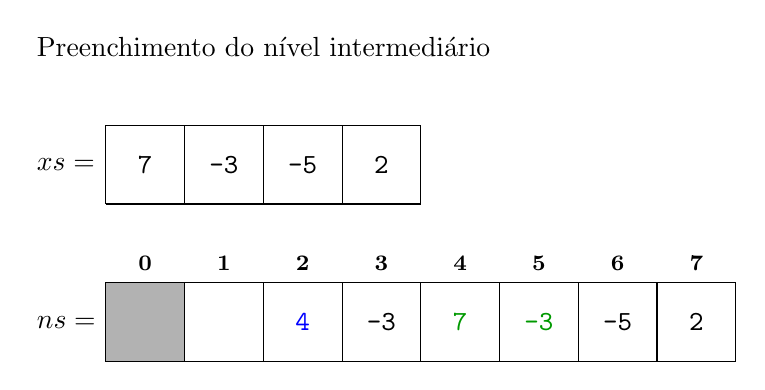
\begin{tikzpicture}
            \node[anchor=west] at (0, 5) { Preenchimento do nível intermediário };
            \node[anchor=west] at (0, 3.5) { $xs =$ };
            \node[anchor=west] at (0, 1.5) { $ns =$ };

            \draw[fill=gray!60] (1, 1) rectangle (2, 2);
            \draw (1, 3) grid (5, 4);
            \draw (1, 1) grid (9, 2);

            \node at (1.5, 2.25) { \footnotesize $\mathtt{\mathbf{0}}$ };
            \node at (2.5, 2.25) { \footnotesize $\mathtt{\mathbf{1}}$ };
            \node at (3.5, 2.25) { \footnotesize $\mathtt{\mathbf{2}}$ };
            \node at (4.5, 2.25) { \footnotesize $\mathtt{\mathbf{3}}$ };
            \node at (5.5, 2.25) { \footnotesize $\mathtt{\mathbf{4}}$ };
            \node at (6.5, 2.25) { \footnotesize $\mathtt{\mathbf{5}}$ };
            \node at (7.5, 2.25) { \footnotesize $\mathtt{\mathbf{6}}$ };
            \node at (8.5, 2.25) { \footnotesize $\mathtt{\mathbf{7}}$ };

            \node at (1.5, 3.5) { \tt 7 };
            \node at (2.5, 3.5) { \tt -3 };
            \node at (3.5, 3.5) { \tt -5 };
            \node at (4.5, 3.5) { \tt 2 };

            \node at (3.5, 1.5) { \tt \textcolor{blue}{4} };
            \node at (4.5, 1.5) { \tt \textcolor{black}{-3} };
            \node at (5.5, 1.5) { \tt \textcolor{green!60!black}{7} };
            \node at (6.5, 1.5) { \tt \textcolor{green!60!black}{-3} };
            \node at (7.5, 1.5) { \tt \textcolor{black}{-5} };
            \node at (8.5, 1.5) { \tt \textcolor{black}{2} };
        \end{tikzpicture}
    \end{figure}

\end{frame}

\begin{frame}[fragile]{Visualização do construtor da árvore de segmentos}

    \begin{figure}
        \centering

        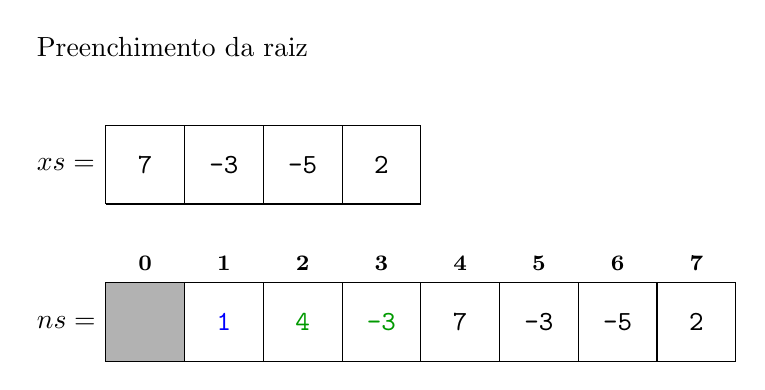
\begin{tikzpicture}
            \node[anchor=west] at (0, 5) { Preenchimento da raiz };
            \node[anchor=west] at (0, 3.5) { $xs =$ };
            \node[anchor=west] at (0, 1.5) { $ns =$ };

            \draw[fill=gray!60] (1, 1) rectangle (2, 2);
            \draw (1, 3) grid (5, 4);
            \draw (1, 1) grid (9, 2);

            \node at (1.5, 2.25) { \footnotesize $\mathtt{\mathbf{0}}$ };
            \node at (2.5, 2.25) { \footnotesize $\mathtt{\mathbf{1}}$ };
            \node at (3.5, 2.25) { \footnotesize $\mathtt{\mathbf{2}}$ };
            \node at (4.5, 2.25) { \footnotesize $\mathtt{\mathbf{3}}$ };
            \node at (5.5, 2.25) { \footnotesize $\mathtt{\mathbf{4}}$ };
            \node at (6.5, 2.25) { \footnotesize $\mathtt{\mathbf{5}}$ };
            \node at (7.5, 2.25) { \footnotesize $\mathtt{\mathbf{6}}$ };
            \node at (8.5, 2.25) { \footnotesize $\mathtt{\mathbf{7}}$ };

            \node at (1.5, 3.5) { \tt 7 };
            \node at (2.5, 3.5) { \tt -3 };
            \node at (3.5, 3.5) { \tt -5 };
            \node at (4.5, 3.5) { \tt 2 };

            \node at (2.5, 1.5) { \tt \textcolor{blue}{1} };
            \node at (3.5, 1.5) { \tt \textcolor{green!60!black}{4} };
            \node at (4.5, 1.5) { \tt \textcolor{green!60!black}{-3} };
            \node at (5.5, 1.5) { \tt \textcolor{black}{7} };
            \node at (6.5, 1.5) { \tt \textcolor{black}{-3} };
            \node at (7.5, 1.5) { \tt \textcolor{black}{-5} };
            \node at (8.5, 1.5) { \tt \textcolor{black}{2} };
        \end{tikzpicture}
    \end{figure}

\end{frame}
